
\begin{frame}{Mutation of a subtree}
\begin{columns}
\begin{column}{0.45\textwidth}
\begin{block}{Before}
\begin{center}
\resizebox{1\textwidth}{!}{%
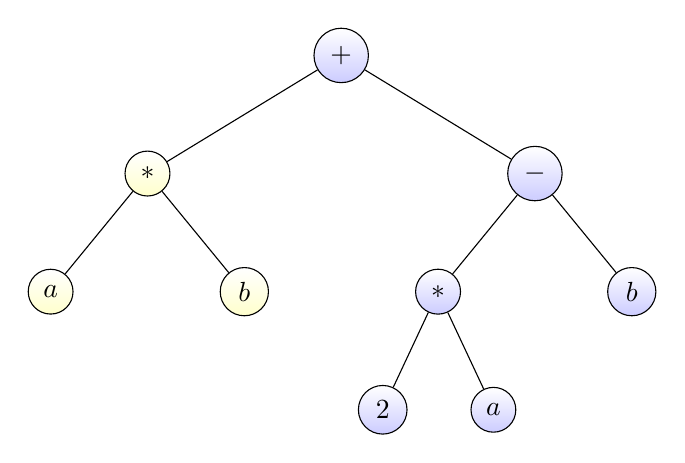
\begin{tikzpicture}[
  every node/.style = {shape=circle,
    draw, align=center,
    top color=white, bottom color=blue!20},
  outro/.style  = { bottom color = yellow!20},
  level 1/.style={sibling distance=14em},
  level 2/.style={sibling distance=7em},
  level 3/.style={sibling distance=4em},
  level 4/.style={sibling distance=2em}]
\node{$+$}
child{
 node[outro]{$*$}
 child{
  node[outro]{$a$}
  }
  child{
  node[outro]{$b$}
  }
 }
 child{
 node{$-$}
 child{
  node{$*$}
  child{
   node{$2$}
   }
   child{
   node{$a$}
   }
  }
  child{
  node{$b$}
  }
 }
;
\end{tikzpicture}
}
\end{center}
\end{block}
\end{column}

\begin{column}{0.45\textwidth}
\begin{block}{After}
\begin{center}
\resizebox{0.8\textwidth}{!}{%
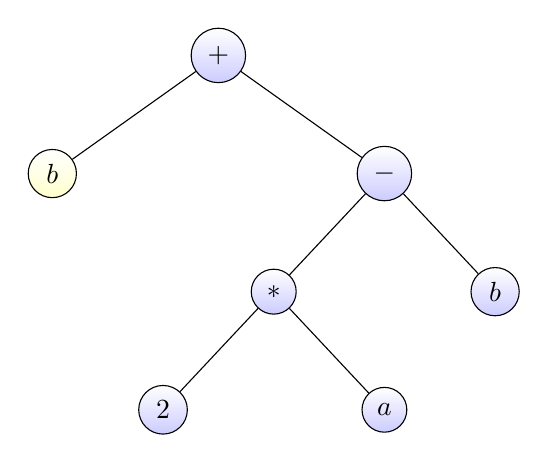
\begin{tikzpicture}[
  every node/.style = {shape=circle,
    draw, align=center,
    top color=white, bottom color=blue!20},
  outro/.style  = { bottom color = yellow!20},
  level 1/.style={sibling distance=12em},
  level 2/.style={sibling distance=8em},
  level 3/.style={sibling distance=8em},
  level 4/.style={sibling distance=8em}]
\node{$+$}
child{
  node[outro]{$b$}
 }
 child{
 node{$-$}
 child{
  node{$*$}
  child{
   node{$2$}
   }
   child{
   node{$a$}
   }
  }
  child{
  node{$b$}
  }
 }
;
\end{tikzpicture}
}
\end{center}
\end{block}
\end{column}
\end{columns}
\end{frame}

\begin{frame}{Mutation of a node}
\begin{columns}
\begin{column}{0.45\textwidth}
\begin{block}{Before}
\begin{center}
\resizebox{1\textwidth}{!}{%
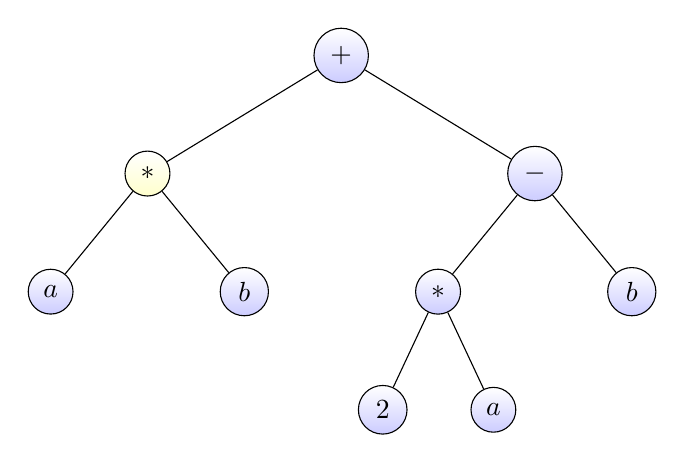
\begin{tikzpicture}[
  every node/.style = {shape=circle,
    draw, align=center,
    top color=white, bottom color=blue!20},
  outro/.style  = { bottom color = yellow!20},
  level 1/.style={sibling distance=14em},
  level 2/.style={sibling distance=7em},
  level 3/.style={sibling distance=4em},
  level 4/.style={sibling distance=2em}]
\node{$+$}
child{
 node[outro]{$*$}
 child{
  node{$a$}
  }
  child{
  node{$b$}
  }
 }
 child{
 node{$-$}
 child{
  node{$*$}
  child{
   node{$2$}
   }
   child{
   node{$a$}
   }
  }
  child{
  node{$b$}
  }
 }
;
\end{tikzpicture}
}
\end{center}
\end{block}
\end{column}

\begin{column}{0.45\textwidth}
\begin{block}{After}
\begin{center}
\resizebox{0.8\textwidth}{!}{%
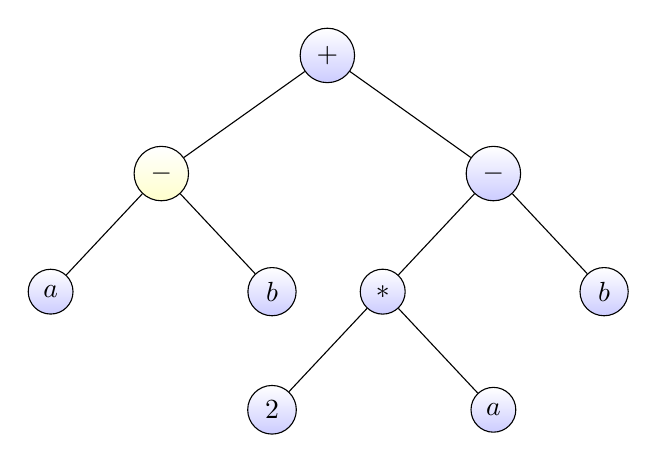
\begin{tikzpicture}[
  every node/.style = {shape=circle,
    draw, align=center,
    top color=white, bottom color=blue!20},
  outro/.style  = { bottom color = yellow!20},
  level 1/.style={sibling distance=12em},
  level 2/.style={sibling distance=8em},
  level 3/.style={sibling distance=8em},
  level 4/.style={sibling distance=8em}]
\node{$+$}
child{
 node[outro]{$-$}
 child{
  node{$a$}
  }
  child{
  node{$b$}
  }
 }
 child{
 node{$-$}
 child{
  node{$*$}
  child{
   node{$2$}
   }
   child{
   node{$a$}
   }
  }
  child{
  node{$b$}
  }
 }
;
\end{tikzpicture}
}
\end{center}
\end{block}
\end{column}
\end{columns}
\end{frame}
